\documentclass[11pt]{article}

\usepackage{geometry}
\usepackage{subcaption} 
\geometry{letterpaper}

\usepackage{doc}
\usepackage{cite}
\usepackage[margin=1cm]{caption}

\usepackage{url}

\usepackage{graphicx}
\usepackage{epstopdf}
\DeclareGraphicsRule{.tif}{png}{.png}{`convert #1 `dirname #1`/`basename #1 .tif`.png}

\title{Dream Design}
\author{Trixie Roque}
\date{11/24/2015}

\begin{document}
\maketitle

\begin{abstract}
The purpose of this paper is to design a new user interface for the Instagram application by integrating timeline options similar to the ones employed by Facebook, as well as allowing the users more freedom in editing their posts. Implementing these features would require integrating other APIs, such as Google Maps, for its ability to create a travel history for the user, and Snapchat, for its ability to grant users the option to doodle on their captured photos. The goal of the interface is to present the user with the power to map out a story based on their travel destination posts. The five usability metrics that are involved, therefore, in the creation of this design idea are learnability, efficiency, and satisfaction.
\end{abstract}

\pagebreak
\tableofcontents

\pagebreak

\section{Introduction}
\label{Introduction}
   \indent 
    \indent Social media applications have become a common tool in our society, especially to millennials. The ability to connect with both friends and strangers alike through the submission of "posts" onto the internet has become so widespread that it is rare to find a person that does not own at least one social media account. Social media has been a gateway for people to communicate by sending clever quips, funny memes, and/or embarrassingly hilarious gifs or videos, among other things. Some people can even say that their hobbies involve sifting through countless blogs, tweets, videos, etc. of internet denizens. Because these social media applications provide us with the capability to peek through the various adventures in other people's lives, we have become incredibly immersed in them. However, even with the continuous appearance of these applications that aim to grab our everyday attention, design improvements are always necessary to cater to the growing number of social media consumers. \\ \\
     \indent In addition to these applications, touchscreen devices have also become a norm. The iPhone, for example, though invented only 8 years ago, has quickly become a popular mobile device for the masses. Phones, in general, have actually evolved into a multi-purpose tool in our everyday lives. Utilizing touch-capable mobile handheld devices as its main system might have even caused the boom in the usage of social media applications. \\ \\
     \indent In this paper, I will focus on a specific social media, one that is mainly used to post pictures for other people to see, called Instagram, focusing on the application that is downloaded through a mobile touch-enabled phone.
     
\section{System Description}
\label{System Description}
   \indent 
   \indent Although there is also a desktop client for Instagram, called Webstagram, the main focus of this paper is to address the designs in the mobile application. There is no question that Instagram would be used more frequently through a phone its main appealing quality is its capability to quickly post snapshots in a matter of seconds. A user can easily choose an already existing picture in their camera roll and tap on a few buttons and their pictures can be viewed by their followers. Additionally, users have the option of taking a picture from within the application so that they do not have to switch between it and the built-in camera application in their device. In addition to the picture, the user is also given an option to write a quick description about the image. \\ \\
   \indent The current design of Instagram appears to be already simplistic, which makes it very intuitive to new users. In the interface, users can scroll through their "news" feed, which contains recent posts of users they follow, or they can take a picture themselves and post it on their feed. Figure 1a shows some available tools for the user after they had just taken a picture. Additionally, the user can also "tag" the location where they took that photo. Figure 1b gives a map of the area where a photo was taken and marks those significant places with the corresponding pictures. For example, in Figure 1b, three pictures were taken near Chiu Tam Path, Hong Kong. The availability of this kind of map gives the user a more visual overview of the places they had visited in the past. 
   
\begin{figure}
\centering
\begin{subfigure}[b]{.5\textwidth}
   \centering
    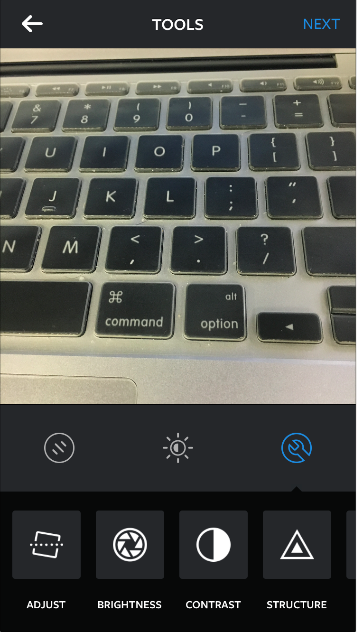
\includegraphics[height=\textwidth]{images/instagram_tools.png}
    \caption{Some tools that exist in Instagram's interface include brightness adjustments.}
    \label{tools}
\end{subfigure}%
~~~~~~~
\begin{subfigure}[b]{.5\textwidth}
    \centering
    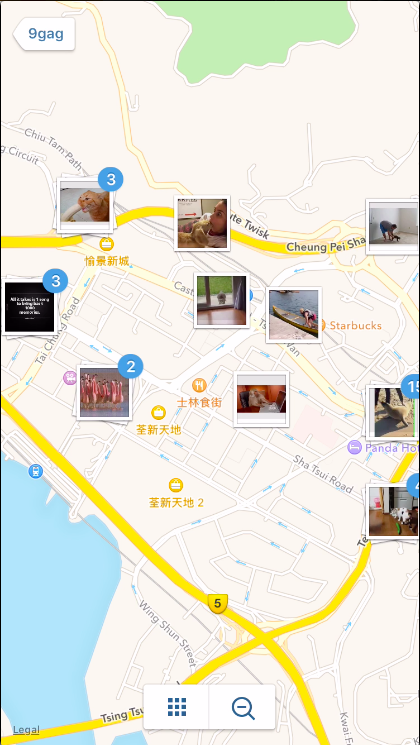
\includegraphics[height=\textwidth]{images/maps_with_pictures.png}
    \caption{Instagram allows users to group pictures based on where they were taken.}
    \label{instagram_pictures}
\end{subfigure}
\caption{Some features available in the Instagram interface}
\end{figure}


\section{Top-Level Design}
\label{Top-Level Design}
   \indent 
   \indent The design would incorporate the Google Maps API and the Instagram API into a conglomeration that allows for posts, as well as 
   \\ \\
   \indent The application will employ Snapchat's feature that allows the user to draw on the images. Currently, Instagram only allows various filters other lighting adjustments
    \\
\begin{figure}[ht]
\centering
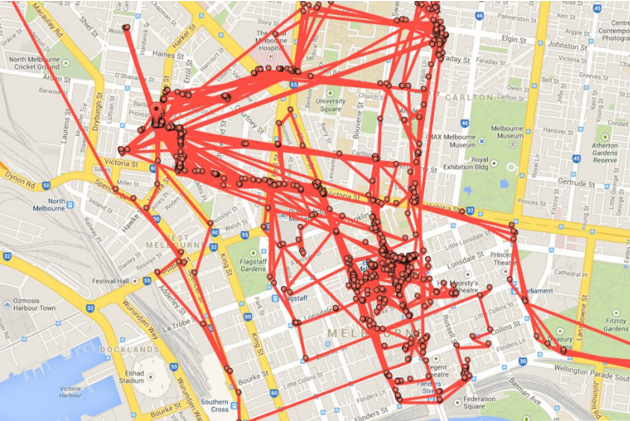
\includegraphics[width=5in]{images/google_maps_tracking.png}
\caption{Google Maps tracks users' travel history}
\label{google_tracking}
\end{figure}

\begin{figure}[ht]
\centering
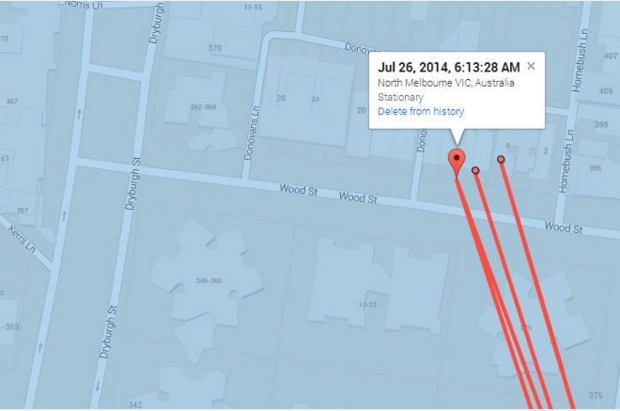
\includegraphics[width=5in]{images/google_maps_tracking_with_info.png}
\caption{The new interface would give the options to view information about the event or delete it.}
\label{google_tracking}
\end{figure}

\begin{figure}[ht]
\centering
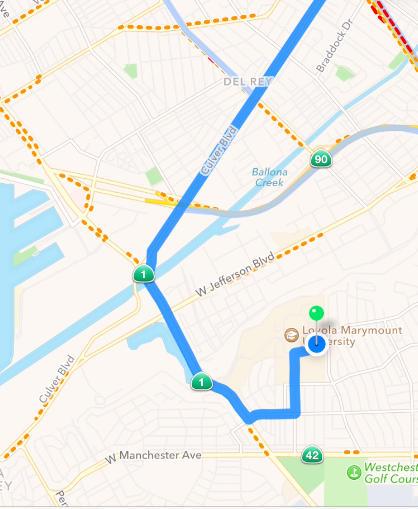
\includegraphics[width=3in]{images/gps.png}
\caption{Google Maps tracks users' travel history.}
\label{travel_history}
\end{figure}

\begin{figure}[ht]
\centering
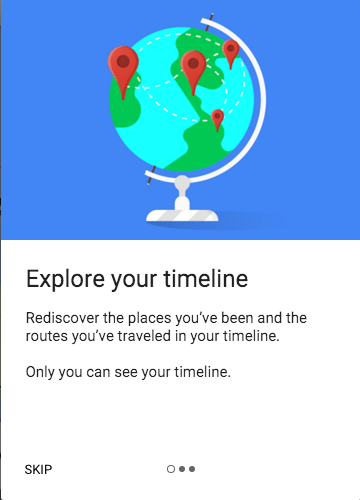
\includegraphics[width=3in]{images/view_your_timeline_prompt.png}
\caption{The new design would allow users to view where they have been, according to their posts' location.}
\label{view_timeline}
\end{figure}

\begin{figure}[ht]
\centering
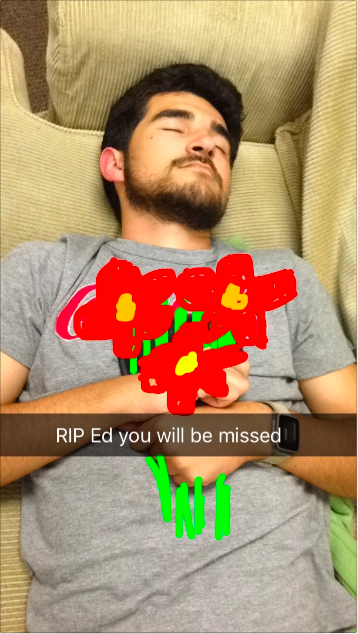
\includegraphics[height=4in]{images/rip_ed.png}
\caption{An example of doodling on a picture. The flowers were hand-drawn directly on the picture.}
\label{ed}
\end{figure}

\section{Usage Scenarios}
\label{Usage Scenarios}
   \indent \\
   \indent The main purpose of the new features in the interface is to allow the user to easily view the places that they have visited. \\


\section{Rationale}
   \indent \\
   \indent The driving force


\section{Usability Metric ``Forecast''}
   \indent 
   \indent Since the new design would integrate features that other APIs present, the usability metrics would have to be discussed in order to keep in mind how the user would interact with the interface. If the designs are successfully implemented and tested, given enough time, money, and manpower, the strongest metrics, as discussed in class, would be satisfaction and learnability. In contrast, the metrics that might suffer from the implementation would be the error and memorability metrics.\\ \\
   \indent Because the purpose of the interface is to allow the users more freedom for their posts, consumer satisfaction is a necessary metric to fulfill. The ability to generate a path containing the places that a person has visited would allow them to both keep a record of their journeys, as well as revisit their old memories of those journeys through a map like interface. With respect to doodling using the touch interface, Additionally, since the interface would be implemented into a social media application, if it becomes widely used, then an expert user can easily navigate through the application's optional features.\\ \\
   \indent Because of the added features, the likelihood that the user encounters errors would definitely increase since the user would have more options to tap a button they did not intend to select. \\ \\
   \indent With respect to the feature that allows the user to draw on the pictures, learnability is an obvious usability metric that is \\

\clearpage

\bibliographystyle{plain}
\end{document}

\end{document}